\chapter{Testování výsledného řešení}
Testování probíhalo pravidelně v průběhu vývoje rozšíření na jednoduchých fragmentech kódu Monkey C jazyka. Pro finální testovaní však byly použity programy, jenž byly součástí reálných aplikací. Tyto příkladové aplikace byly převzaty z oficiální Connect IQ SKD.\\

První testovací zdrojový kód je možné vidět na výpisu \textbf{\ref{testSrc1:Sensor}}. Tento kód komunikuje se senzory obsažených v Garmin zařízení a s jejich pomocí měří srdeční tep uživatele. Při testování tohoto kódu nedošlo k žádným výraznějším problémům. Při deklaraci jednotlivých tříd, které vždy byly rozšířeny jinou třídou pomocí \textbf{extends}, rozšíření správně našeptávalo možné kandidáty na doplnění. Dále ve funkci \textit{initialize()}, kde je volána metoda \textit{enableSensorEvents()}, bylo rozšíření schopno našeptávat callback funkce po zadání znaku '\textbf{:}'. Některé části kódu bylo však nutné upravit. Jako první bylo nutné přidat komentáře s datovým typem nad deklarace proměnných\textit{ stringHR} a \textit{HRgraph}. Zde však nastal problém, kdy nebylo možné jednoznačně určit, jaký datový typ má proměnná \textit{HRgraph} obsahovat. Ve funkci \textit{initialize()} je do této proměnné vložena instance třídy \textbf{LineGraph}. Tuto třídu však rozšíření nenašlo a po zkontrolování oficiální Monkey C API \cite{api_docs} dokumentace bylo zjištěno, že takovou třídu API neobsahuje, tudíž ji rozšíření ani nemohlo nabídnout, jako kandidáta na doplnění.
\\
Druhý testovací zdrojový kód je možné vidět na výpisu \textbf{\ref{testSrc2:BurstChnl}}. Jedná se o část aplikace GenericChannelBurst, která pracuje s třídami Toybox.Ant.BurstListener, Toybox.Ant.Ant.GenericChannel,  Toybox.Ant.ChannelAssignment, atd... U toho zdrojového kódu byl kladen důraz především na práci s konstantami. Hned před deklarací třídy \textit{BurstChannel} lze vidět první konstantu \textbf{ANT-DATA-PACKET-SIZE}. Další konstanty následují již v těle třídy. Na obrázku \ref{img:constants} lze vidět, jak rozšíření našeptává konstanty obsahující písmeno \textbf{D}. Lze si také všimnout, že i lokální proměnné deklarované uživatelem obsahují vlastní popis. V tomto případě je součástí popisu datový typ proměnné. Při importovaní modulů pomocí \textbf{using}, deklaraci třídy společně s použití dědičnosti a deklaraci všech proměnných nebyl detekován žádný problém. Dále byla testována deklarace nového pole, práce s \textbf{for} cyklem, volaní metod na proměnných atd... 

\begin{figure}[tbh!]
	\centering
	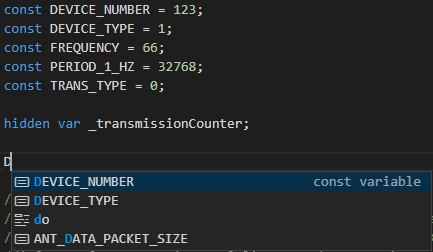
\includegraphics[width=\textwidth,scale=1]{images/constants}
	\caption{rozšíření našeptává konstanty obsahující písmeno D.}
	\label{img:constants}
\end{figure}